
\documentclass[../../../all/physics-standard_answers_all.tex]{subfiles}

\graphicspath{{../../../../figures/}}

\begin{document}

\setlength{\abovedisplayskip}{2mm}
\setlength{\belowdisplayskip}{1mm}

\begin{enumerate}

    \item 電気力線は等電位線に直交し，高電位から低電位へ向かう向きである．
        %
        \par \vspace{0.2\baselineskip}
        {\centering
            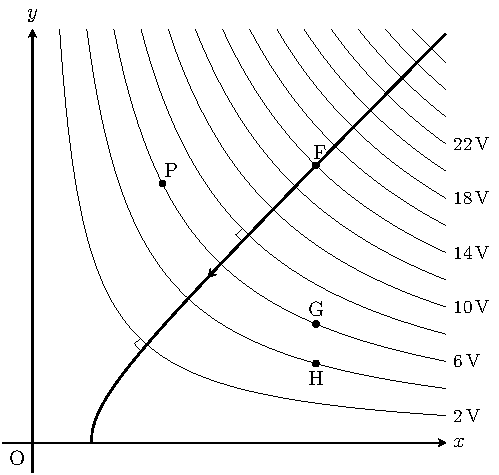
\includegraphics{a_electric-field_09_01/physics-standard_answers_electric-field_09_01_tikz.pdf}
        \par}
        \vspace{0.2\baselineskip}

    \item 電場は電位の空間勾配に等しいので，
        %
        \begin{align*}
            E_\mathrm{F} \fallingdotseq \frac{2 \, \mathrm{V}}{0.38 \, \mathrm{m}}
            = 5.26 \cdots \, \mathrm{V/m} \fallingdotseq \uwave{5.3 \, \mathrm{V/m}} \;.
        \end{align*}
     
\end{enumerate}

\end{document}
